\section{Experimental Results and Analyses}
\label{sec:results}

\paragraph{Main Results}
We report the main results in Table~\ref{tab:main}, where OmniRetrieval consistently outperforms all baselines across the five backbones. The four single-backend baselines, each pinned to one paradigm, perform poorly since three of the four query types lie outside their reach. KB Routing lifts this restriction by routing to one source per query, but its up-front commitment leaves no fallback when the chosen source is wrong. OmniRetrieval instead engages multiple candidates and consolidates them via cross-source evidence selection, yielding consistent gains over KB Routing. Also, the gap to the Oracle upper bound narrows from selection to judge ($34.27 \to 17.51 \to 8.67$ pts), suggesting that evidence selection often recovers a semantically equivalent answer from an alternative source even when source selection misses.

\begin{figure*}[t!]
    \centering
    \begin{minipage}[t]{0.70\linewidth}
        \centering
        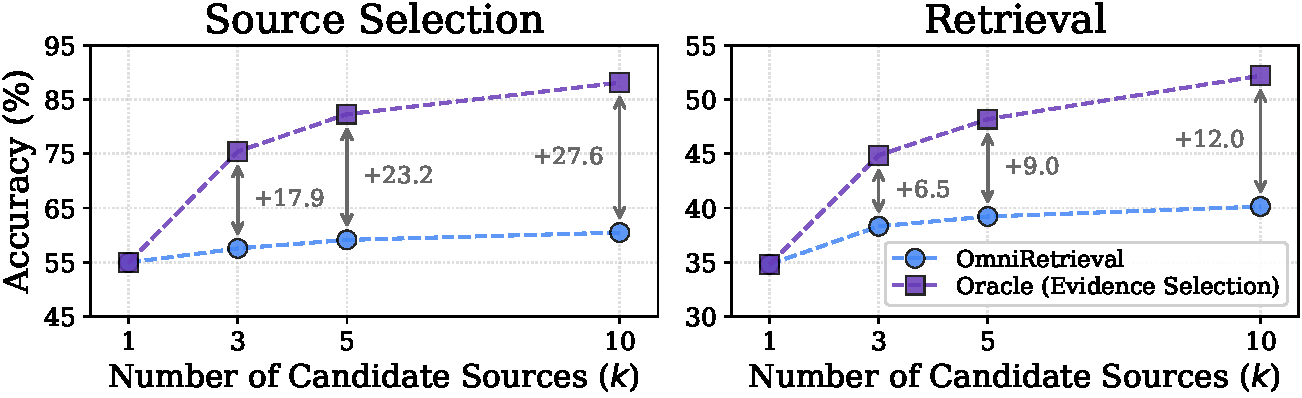
\includegraphics[width=0.975\linewidth]{figures/topk_sweep_fig.pdf}
        \vspace{-0.1in}
        \captionof{figure}{Effect of the candidate list size $k$ in source selection on Source Selection and Retrieval accuracy. \textbf{Oracle (Evidence Selection)} replaces the LLM-based evidence selection with gold-source selection within the top-$k$ candidates.}
        \label{fig:topk_sweep}
    \end{minipage}
    \hfill
    \begin{minipage}[t]{0.28\linewidth}
        \centering
        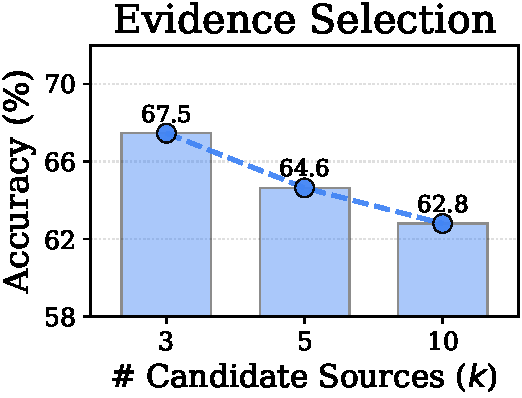
\includegraphics[width=0.975\linewidth]{figures/selector_analysis_fig.pdf}
        \vspace{-0.1in}
        \captionof{figure}{Evidence-selection accuracy on multi-candidate questions with the gold in the top-$k$.}
        \label{fig:selector_analysis}
    \end{minipage}
\end{figure*}

\begin{figure*}[t!]
    \centering
    \begin{minipage}[t]{0.70\linewidth}
        \centering
        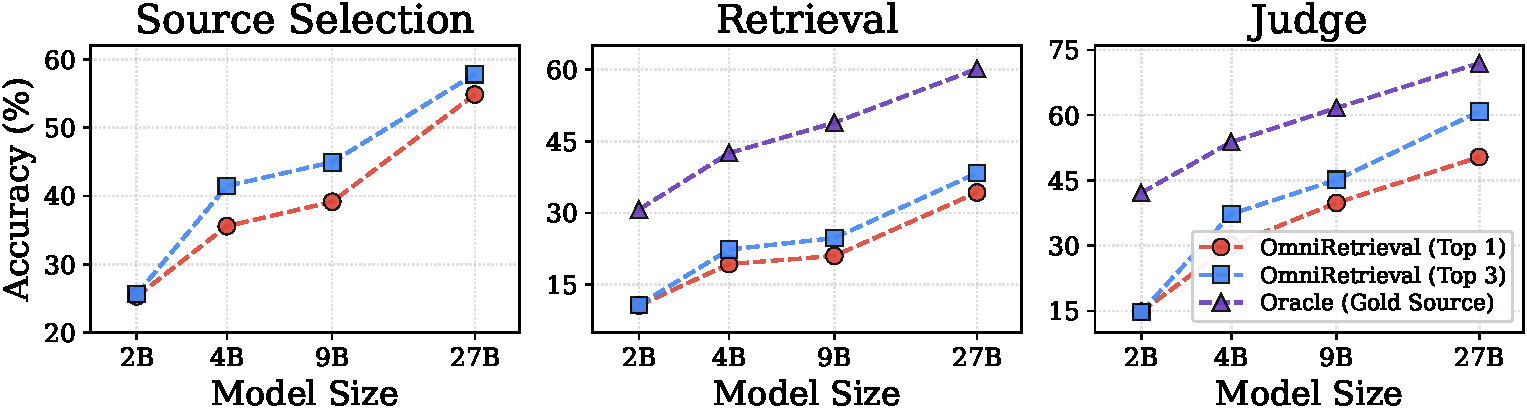
\includegraphics[width=0.975\linewidth]{figures/qwen_scaling_fig.pdf}
        \vspace{-0.1in}
        \captionof{figure}{Effect of backbone scale (Qwen-3.5, 2B to 27B). \textbf{Oracle (Gold Source)} uses the gold source in place of LLM-based source selection, and is omitted from Source Selection (where it is trivially $100\%$ by construction).}
        \label{fig:qwen_scaling}
    \end{minipage}
    \hfill
    \begin{minipage}[t]{0.28\linewidth}
        \centering
        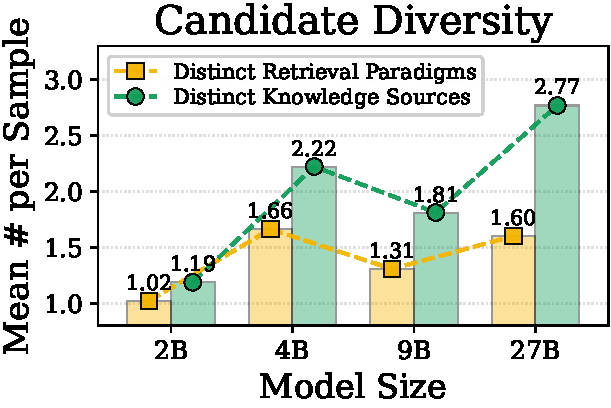
\includegraphics[width=0.975\linewidth]{figures/qwen_diversity_fig.pdf}
        \vspace{-0.1in}
        \captionof{figure}{Candidate diversity: distinct retrieval paradigms and knowledge sources per sample.}
        \label{fig:qwen_diversity}
    \end{minipage}
\end{figure*}


\paragraph{Analysis on Source Candidate Size}
Recall that the source-selection step of OmniRetrieval returns a short list of $k$ candidate sources, which is then fed into per-source query formulation and cross-source evidence selection. To see its effect, we sweep $k \in \{1, 3, 5, 10\}$ with Qwen-3.5 (27B) and additionally compare against an \textbf{Oracle (Evidence Selection)} variant that replaces the LLM-based selector with gold-source selection within the $k$. As shown in Figure~\ref{fig:topk_sweep}, OmniRetrieval improves monotonically with $k$, yet the oracle improves much faster, widening the gap to the oracle as $k$ grows. This observation traces to the selector itself: its multi-candidate 1-of-$k$ accuracy drops from $67.5\%$ at $k{=}3$ to $62.8\%$ at $k{=}10$ (Figure~\ref{fig:selector_analysis}). Thus, combined with the linear cost of additional candidates, this points to the initial evidence selection as the more impactful lever.

\paragraph{Analysis on Backbone Scale}
Building on the analysis above, we next vary the backbone scale by sweeping Qwen-3.5 from $2$B to $27$B, comparing OmniRetrieval (Top 1, one candidate per question) with OmniRetrieval (Top 3, our default). As shown in Figure~\ref{fig:qwen_scaling}, the two are essentially tied at 2B and Top 3 takes a clear lead at 27B, a gap that traces to candidate diversity (Figure~\ref{fig:qwen_diversity}): at 2B the source-selection step collapses to a single paradigm, while beyond 4B it produces meaningfully different candidates across both paradigms and sources\footnote{Qwen-3.5 9B exhibits a bias toward Document Search at its top candidate, pulling its candidates into the same retrieval paradigm; this surfaces as the diversity dip in Figure~\ref{fig:qwen_diversity}.}. Yet the gap to Oracle (Gold Source) ceiling remains, the largest on Source Selection, underscoring source selection as the most consequential step in the pipeline. This aligns with the design rationale of OmniRetrieval: broad exploration at source-selection, with the final commitment deferred to the evidence-selection.

\begin{figure*}[t!]
    \centering
    \begin{minipage}[t]{0.36\linewidth}
        \vspace{0pt}
        \centering
        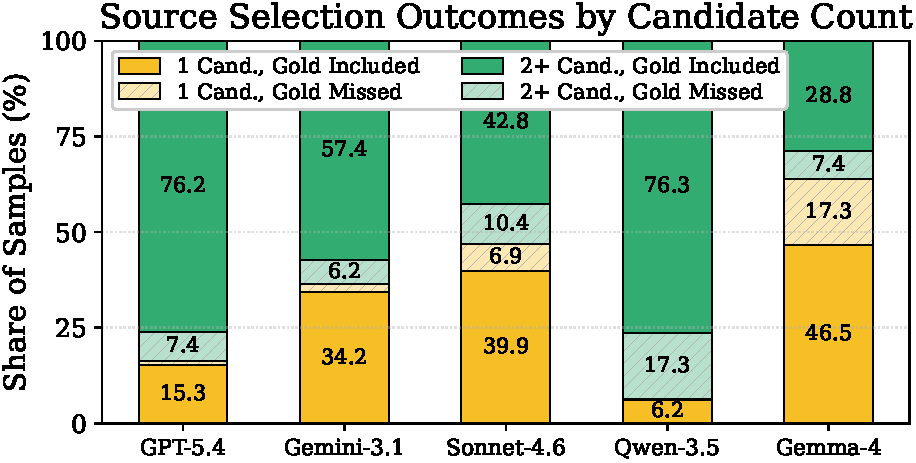
\includegraphics[width=0.98\linewidth]{figures/cross_backbone_selector_fig.pdf}
        \vspace{-0.11in}
        \captionof{figure}{Source-selection behavior on 1 and 2+ candidate regimes. Solid segments mark success (gold present in the candidate list); hatched ones mark failure.}
        \label{fig:cross_backbone_selector}
    \end{minipage}
    \hfill
    \begin{minipage}[t]{0.315\linewidth}
        \vspace{0pt}
        \centering
        \captionof{table}{Evidence-selection accuracy on multi-candidate questions containing the gold, where \textit{Random} is the per-backbone uniform-pick baseline.}
        \label{tab:evidence_selection}
        \vspace{-0.05in}
        \resizebox{\linewidth}{!}{%
        \setlength{\tabcolsep}{2.5pt}
        \renewcommand{\arraystretch}{1.25}
        \begin{tabular}{l c c c}
            \toprule
            \textbf{Backbone} & \textbf{Acc. (\%)} & \textbf{Rand. (\%)} & \textbf{$\Delta$ (pp)} \\
            \midrule
            GPT-5.4    & 72.81 & 38.31 & $+34.51$ \\
            Gemini-3.1 & 75.29 & 43.99 & $+31.30$ \\
            Sonnet-4.6 & 70.44 & 41.47 & $+28.98$ \\
            Qwen-3.5   & 67.91 & 35.55 & $+32.36$ \\
            Gemma-4    & 74.33 & 47.73 & $+26.60$ \\
            \bottomrule
        \end{tabular}%
        }
    \end{minipage}
    \hfill
    \begin{minipage}[t]{0.30\linewidth}
        \vspace{0pt}
        \centering
        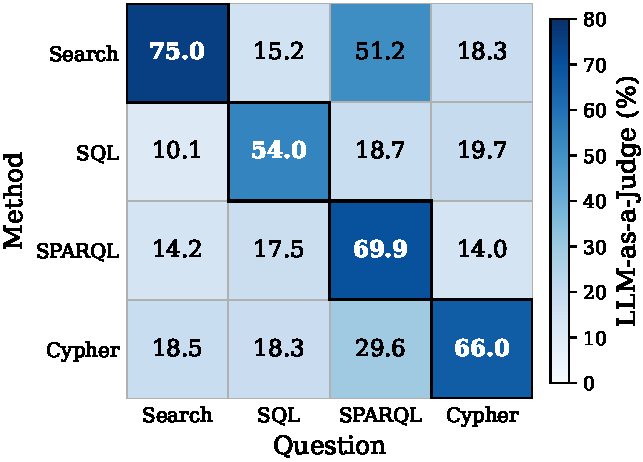
\includegraphics[width=0.95\linewidth]{figures/paradigm_coverage_fig.pdf}
        \vspace{-0.11in}
        \captionof{figure}{LLM-Judge accuracy on GPT-5.4 (rows: method paradigm; columns: question paradigm).}
        \label{fig:paradigm_coverage}
    \end{minipage}
\end{figure*}


\paragraph{Analysis on Cross-Source Evidence Selection}
Building on the prior deferral argument, we examine how reliably evidence selection commits to the gold candidates. The source-selection step lands in one of two regimes per question, either committing to a single candidate or emitting two or more, and the exploration versus commitment trade-off varies widely across backbones (Figure~\ref{fig:cross_backbone_selector}). Yet two patterns hold consistently. First, the gold source is included in the candidate list at a high rate at every backbone. Second, once included, the evidence-selection step picks it at a high rate as well, far above the per-backbone random baseline (Table~\ref{tab:evidence_selection}). Broad upstream exploration thus translates into accurate final commitments at the step that follows.

\paragraph{Analysis on Cross-Paradigm Coverage}
To see how much of the question space each paradigm can cover, Figure~\ref{fig:paradigm_coverage} reports a matrix of LLM-as-a-Judge accuracy on GPT-5.4, with rows as the method paradigm and columns as the question paradigm. From this, we find that Document Search has by far the widest cross-paradigm coverage, with an off-diagonal mean of $28.2\%$ against $15.2$ to $22.1\%$ for the three structured paradigms. The advantage is largely driven by SPARQL questions, where the Wikipedia-derived corpora exposed under Search overlap with the factual content of Wikidata.

\providecolor{mygray}{HTML}{F2F2F2}
\providecolor{citeblue}{HTML}{1668b0}

\begin{wraptable}{r}{0.45\textwidth}
    \vspace{-0.20in}
    \centering
    \caption{
    Results for the unified-representation methods~\citep{UniK, UDT} with the constrained setup on GPT-5.4, marked $^\dagger$ as non-comparable.
    }
    \label{tab:constrained_baseline}
    \vspace{-0.075in}
    \small
    \resizebox{\linewidth}{!}{
    \setlength{\tabcolsep}{3pt}
    \renewcommand{\arraystretch}{1.1}
    \begin{tabular}{l c c c}
        \toprule
        \textbf{Method} & \textbf{Source Sel.} & \textbf{Retrieval} & \textbf{Judge} \\

        \midrule

        Document Search                              & 21.49 & 13.42 & 39.93 \\
        Unified Representation$^\dagger$             & 31.00 & 23.00 & 45.00 \\
        KB Routing                                   & \underline{64.88} & \underline{42.07} & \underline{60.26} \\
        \rowcolor{citeblue!10}
        \textbf{OmniRetrieval (Ours)}                & \textbf{68.58} & \textbf{46.62} & \textbf{69.72} \\

        \bottomrule
    \end{tabular}
    }
    \vspace{-0.1in}
\end{wraptable}

\paragraph{Analysis on Native vs Unified Retrieval}
To examine how shared-representation methods would perform once the pool is shrunk to a scale they can index (via sub-sampling), we build a constrained pool that retains only the gold-touched triples and edges in SPARQL and Cypher (with a same-count random distractor), includes all SQL tables, and keeps the document corpus at full scale. All items are verbalized and embedded into a single space with \texttt{all-MiniLM-L6-v2}, and the top-3 retrievals, matched to the candidate budget of OmniRetrieval, serve as the final results. As shown in Table~\ref{tab:constrained_baseline}, the unified method surpasses the four single-backend baselines through occasional cross-paradigm coverage, but stays far below KB Routing and OmniRetrieval. The gap persists even though the constrained setting hands this unified method an advantage no other method receives, pointing to a fundamental limit: atomic-unit retrieval cannot capture the structural composition (e.g., joins, traversals, multi-hop chains) that native queries express.
